% ----- Fonctionnement -----

\subsection{How it works}

    To explain how our algorithm works, we will keeps track of two groups of vertices : $S$ which is a partially constructed (non-maximal) clique and the partial solution that we will gradually implement. Moreover, we got $P$  which is the candidates vertices that could be included in the clique, and which represents the union of all vertex neighbors of the vertices in $S$. Furthermore, we got $W$ which is the total weight of $S$ that we will implement
    \\ \\
    The algorithm begins by identifying the vertex with the highest sum of weights of its edges. If there are multiple vertices with the same maximum sum, the vertex with the highest degree is selected. The selected vertex is then added to $S$ and its neighbors are added to $P$. Then the algorithm selects a new vertex from the candidates set $P$ and adds it to $S$. We add to $W$ the weight of the edge between the new vertex selected and every vertices in $S$. This selected vertex is the one with the most weighted edge among all the vertices in $P$. After this step, $P$ is updated by considering only the neighbors of the vertices that are already part of $S$, and by excluding the vertices that are already part of $S$ from $P$. This process is then repeated until no more vertices are left in $P$, at which point the algorithm has obtained its maximum clique $S$.
    \\ \\
    To illustrate the Constructive algorithm, let's use the example in
    Figure \ref{fig:basic-graph-example} on page \pageref{fig:basic-graph-example} while adding some weight to its edges: \\

    \begin{minipage}{\linewidth}
        \textbf{Step 0:} \newline
        \begin{minipage}{0.4\textwidth}
            \begin{figure}[H]
                \centering
                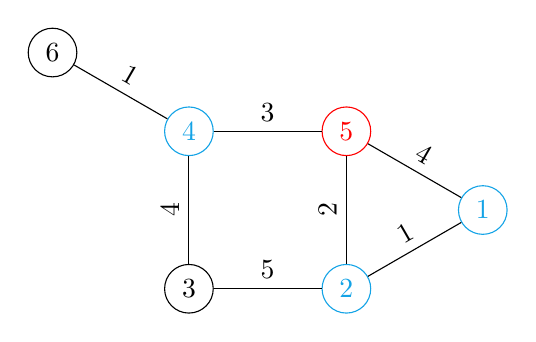
\begin{tikzpicture}[node distance=2cm]
                    \node[circle, draw, Cerulean] (1) {1};
                    \node[circle, draw, Cerulean] (2) at ([shift=(210:2)] 1) {2};
                    \node[circle, draw] (3) [left of=2] {3};
                    \node[circle, draw, Cerulean] (4) [above of=3] {4};
                    \node[circle, draw, red] (5) [above of=2] {5};
                    \node[circle, draw] (6) at ([shift=(150:2)] 4) {6};
    
                    \draw  (1) -- (2) node[midway, above, sloped] {1};
                    \draw (1) -- (5) node[midway, above, sloped] {4};
                    \draw (2) -- (3) node[midway, above, sloped] {5};
                    \draw (2) -- (5) node[midway, above, sloped] {2};
                    \draw (3) -- (4) node[midway, above, sloped] {4};
                    \draw (4) -- (5) node[midway, above, sloped] {3};
                    \draw (4) -- (6) node[midway, above, sloped] {1};
                \end{tikzpicture}
                \caption{Graph illustration for the constructive algorithm at step 0}
                \label{fig:constructive-mewc-edge}
            \end{figure}
        \end{minipage}
        \begin{minipage}{0.6\textwidth}
            At the initial step, as said before, we will initialize $S$, $P$ and $W$ by searching for the vertex with highest sum of weights of its edges $v$ by iterating every vertex on the graph. In this example, we will eventually find 3 and 5 which have a maximum sum of 9. The algorithm will then take the vertex of highest degree between them and will add it to $S$, represented in \textcolor{red}{red}. The neighboring vertex of $v$ will be added to $P$, represented in \textcolor{Cerulean}{blue}.
    
            \begin{center}
                \begin{tabular}{|lll|}
                    \hline
                    S = \{5\} & P = \{1,2,4\} & W = 0 \\
                    \hline
                \end{tabular}
            \end{center}
        \end{minipage}
    \end{minipage} 
    
    \vspace{1\baselineskip}

    \begin{minipage}{\linewidth}
        \textbf{Step 1:} \newline
        \begin{minipage}{0.4\textwidth}
            \begin{figure}[H]
                \centering
                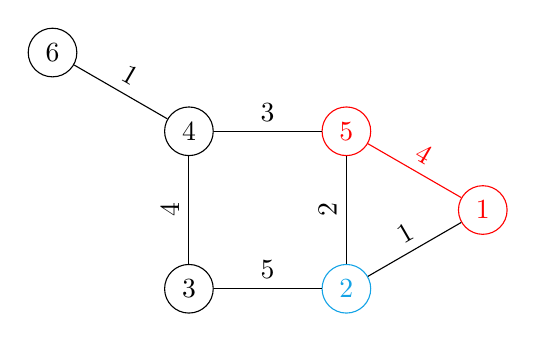
\begin{tikzpicture}[node distance=2cm]
                    \node[circle, draw, red] (1) {1};
                    \node[circle, draw, Cerulean] (2) at ([shift=(210:2)] 1) {2};
                    \node[circle, draw] (3) [left of=2] {3};
                    \node[circle, draw] (4) [above of=3] {4};
                    \node[circle, draw, red] (5) [above of=2] {5};
                    \node[circle, draw] (6) at ([shift=(150:2)] 4) {6};
    
                    \draw  (1) -- (2) node[midway, above, sloped] {1};
                    \draw[red] (1) -- (5) node[midway, above, sloped] {4};
                    \draw (2) -- (3) node[midway, above, sloped] {5};
                    \draw (2) -- (5) node[midway, above, sloped] {2};
                    \draw (3) -- (4) node[midway, above, sloped] {4};
                    \draw (4) -- (5) node[midway, above, sloped] {3};
                    \draw (4) -- (6) node[midway, above, sloped] {1};
                \end{tikzpicture}
                \caption{Graph illustration for the constructive algorithm at step 1}
                \label{fig:constructive-mewc-edge}
            \end{figure}
        \end{minipage}
        \begin{minipage}{0.6\textwidth}
            Then the algorithm will iterate all the neighbors of $v$, and look for the one who shares the edge with the highest weight, which replace $v$ (here 1). If there are several edges with the same weight, the algorithm will take the one with the highest degree. After having found it, we add it to $S$ as well as the weight of the edges of all the vertices in S and $v$ to $W$ (here 4), we update $P$ by keeping only the common neighbors of the members of $S$ (here only 2).
    
            \begin{center}
                \begin{tabular}{|lll|}
                    \hline
                    S = \{5,1\} & P = \{2\} & W = 4 \\
                    \hline
                \end{tabular}
            \end{center}
        \end{minipage}
    \end{minipage} 

    \vspace{1\baselineskip}

    \begin{minipage}{\linewidth}
        \textbf{Step 2:} \newline
        \begin{minipage}{0.4\textwidth}
            \begin{figure}[H]
                \centering
                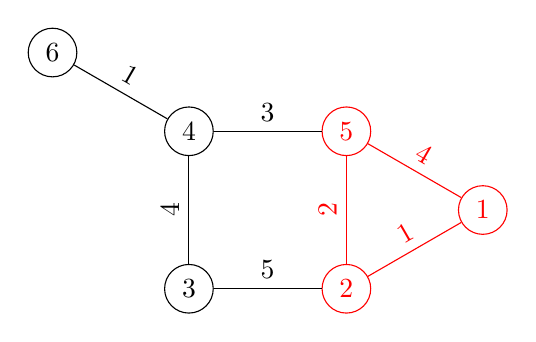
\begin{tikzpicture}[node distance=2cm]
                    \node[circle, draw, red] (1) {1};
                    \node[circle, draw, red] (2) at ([shift=(210:2)] 1) {2};
                    \node[circle, draw] (3) [left of=2] {3};
                    \node[circle, draw] (4) [above of=3] {4};
                    \node[circle, draw, red] (5) [above of=2] {5};
                    \node[circle, draw] (6) at ([shift=(150:2)] 4) {6};
    
                    \draw[red]  (1) -- (2) node[midway, above, sloped] {1};
                    \draw[red] (1) -- (5) node[midway, above, sloped] {4};
                    \draw (2) -- (3) node[midway, above, sloped] {5};
                    \draw[red] (2) -- (5) node[midway, above, sloped] {2};
                    \draw (3) -- (4) node[midway, above, sloped] {4};
                    \draw (4) -- (5) node[midway, above, sloped] {3};
                    \draw (4) -- (6) node[midway, above, sloped] {1};
                \end{tikzpicture}
                \caption{Graph illustration for the constructive algorithm at step 2}
                \label{fig:constructive-mewc-edge}
            \end{figure}
        \end{minipage}
        \begin{minipage}{0.6\textwidth}
            Then, the algorithm will repeat the process of step 1 until $P$ is empty. It will look for a new $v$ (here 2). After finding it, it will add it to $S$ as well as the weight of the edges of all the vertices in $S$ and it to $W$ (here 2 + 1). It will then update $P$ which here will be empty, the algorithm stops and we get the maximum clique in \textcolor{red}{red} and his weight (here (5,1,2) of weight 7).
    
            \begin{center}
                \begin{tabular}{|lll|}
                    \hline
                    S = \{5,1,2\} & P = \{\} & W = 7 \\
                    \hline
                \end{tabular}
            \end{center}
        \end{minipage}
    \end{minipage}

    \vspace{1\baselineskip}

    The constructive algorithm is now finished and we have obtained the following maximum clique of weight 7 : $$(1,2,5)$$

\newpage

